\setboolean{IsHalfPage}{true}%
\setboolean{IsHalfPageLeftCol}{true}%
\setboolean{IsHalfPageRightCol}{false}%
\def\ChapterTitle{%
	Dynamic Metamorphosis
}
\def\ChapterUrl{%
	https://arnottferels.github.io/work/dynamic-metamorphosis
}
\def\ChapterDescription{%
	A fusion of Architectural Innovation \& Interactive Engagement
}
\def\ChapterDetailsLine{%
	Professional Work -- 2021 | Rattan, Surface Exploration, Pattern Generation \& Design
}
\def\ChapterDetailsTabular{%
	\begin{tabular}{@{}ll}
		\textbf{Contributions} & Research and Development, Digital Modeling, Analysis and Simulation \& Scripting \\
		\textbf{Software}      & Rhino \& Grasshopper                                                             \\
		\textbf{Team Leader}   & Trianzani Sulshi                                                                 \\
		\textbf{URL}           & \textcolor{blue}{\footnotesize\texttt{\href{\ChapterUrl}{\ChapterUrl}}}          \\
	\end{tabular}
}
\def\ChapterAbstract{%
	This project centers on refining Seniman Ruang's Hyperbolic Paraboloid design, aiming to optimize both aesthetics and functionality. Leveraging computational tools, the goal is to elevate the unique features of the design, creating an engaging and visually compelling space for visitors. This endeavor reflects a commitment to pushing design boundaries through innovative computational methodologies.
}
\def\ChapterFrontmatter{%
	\chapter*{\ChapterTitle}\addcontentsline{toc}{chapter}{\ChapterTitle}
	\ChapterSetTocAddData{\ChapterDetailsLine}
	\ChapterSetDetailsData{\ChapterDescription}{\ChapterDetailsLine}{\ChapterDetailsTabular}
	\RuleAbstract%
	\ChapterAbstract
}
\StartTwoColumnLayout
\raggedright
\begin{minipage}[t][(\PaperHeight-\PaperTopMargin-\PaperBottomMargin
		-16pt%
		)\relax][t]{\linewidth}%
	\ChapterFrontmatter
	\section*{
	  Ideas
	 }
	\begin{multicols}{2}
		%
\begin{figure}[H]
	\centering
	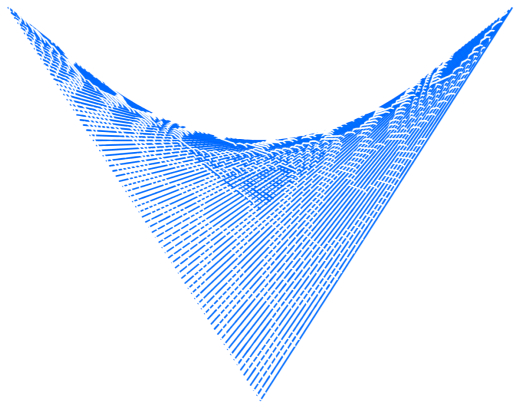
\includegraphics[width=\linewidth]{src/graphics/dynamic-metamorphosis--ideas-form-a.jpg}
	\label{
		fig:dynamic-metamorphosis--ideas-form-a
	}
\end{figure}

		%
\begin{figure}[H]
	\centering
	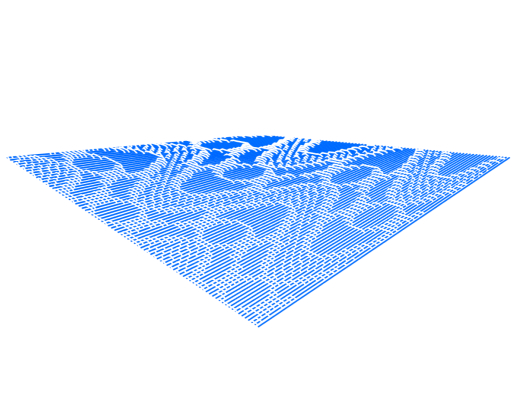
\includegraphics[width=\linewidth]{src/graphics/dynamic-metamorphosis--ideas-form-b.jpg}
	\label{
		fig:dynamic-metamorphosis--ideas-form-b
	}
\end{figure}

	\end{multicols}
	In conceptualizing this transformative project, a multifaceted approach is employed to seamlessly transition between two distinct shapes, Forms A and B. Form A, representing the dynamic Hyperbolic Paraboloid surface, is meticulously crafted to showcase intricate curvatures and fluidity. In contrast, Form B intentionally adopts a predominantly flat surface, creating a deliberate narrative contrast within the design.
	\vspace{\baselineskip}
	\newline%
	Seniman Ruang's forward-thinking grid layout is composed of precisely shaped circular columns, forming the foundational structure for the Hyperbolic Paraboloid. Each column, uniform in thickness, contributes to the creation of a visually striking and static structure. The integration of a basic surface within each grid section, connected with opposing axes, defines the unique character of the Hyperbolic Paraboloid.
	\section*{
	  Method
	 }
	\begin{minipage}[t]{0.65\linewidth}
		%
\begin{figure}[H]
	\centering
	\includesvg[width=\linewidth]{src/graphics/dynamic-metamorphosis--method.svg}
	\label{
		fig:dynamic-metamorphosis--method
	}
\end{figure}

	\end{minipage}
	\hfill
	\begin{minipage}[t]{0.3\linewidth}
		%
\begin{figure}[H]
	\centering
	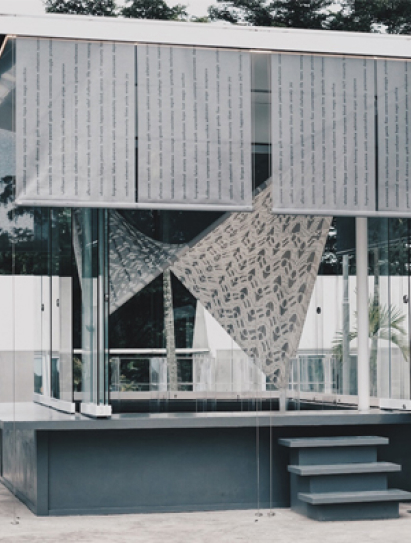
\includegraphics[width=\linewidth]{src/graphics/dynamic-metamorphosis--image.jpg}
	\label{
		fig:dynamic-metamorphosis--image
	}
\end{figure}

	\end{minipage}
	\vfill
	This illustration depicts the gradual shift from Form A to Form B, ranging from 100\% Form A (100:0) to 100\% Form B (0:100). To ensure day-long engagement, advanced methods are employed, including strategically placed motors for smooth Hyperbolic Paraboloid movement, creating a dynamic and interactive focal point during sales activities. These innovative design approaches aim to go beyond the ordinary, fostering enjoyable and intriguing spaces that challenge traditional design norms.
\end{minipage}
\EndTwoColumnLayout
\newpage
